%%%%%%%%%%%%%%%%%%%%%%%%%%%%%%%%%%%%%%%%%%%%%%%%%%%%%%%%%%%%%%%%%%%%%%%%%%%%%%%%
%%%%%%%%%%%%%%%%%%   Vorlage für eine Abschlussarbeit   %%%%%%%%%%%%%%%%%%%%%%%%
%%%%%%%%%%%%%%%%%%%%%%%%%%%%%%%%%%%%%%%%%%%%%%%%%%%%%%%%%%%%%%%%%%%%%%%%%%%%%%%%

% Erstellt von Maximilian Nöthe, <maximilian.noethe@tu-dortmund.de>
% ausgelegt für lualatex und Biblatex mit biber

% Kompilieren mit
% latexmk --lualatex --output-directory=build thesis.tex
% oder einfach mit:
% make

\documentclass[
  tucolor,       % remove for less green,
  BCOR=12mm,     % 12mm binding corrections, adjust to fit your binding
  parskip=half,  % new paragraphs start with half line vertical space
  open=any,      % chapters start on both odd and even pages
  cleardoublepage=plain,  % no header/footer on blank pages
]{tudothesis}


% Warning, if another latex run is needed
\usepackage[aux]{rerunfilecheck}

% just list chapters and sections in the toc, not subsections or smaller
\setcounter{tocdepth}{1}

%------------------------------------------------------------------------------
%------------------------------ Fonts, Unicode, Language ----------------------
%------------------------------------------------------------------------------
\usepackage{fontspec}
\defaultfontfeatures{Ligatures=TeX}  % -- becomes en-dash etc.

% load english (for abstract) and ngerman language
% the main language has to come last
\usepackage[american]{babel}

% intelligent quotation marks, language and nesting sensitive
\usepackage[autostyle]{csquotes}

% microtypographical features, makes the text look nicer on the small scale
\usepackage{microtype}

%------------------------------------------------------------------------------
%------------------------ Math Packages and settings --------------------------
%------------------------------------------------------------------------------

\usepackage{amsmath}
\usepackage{amssymb}
\usepackage{mathtools}

% Enable Unicode-Math and follow the ISO-Standards for typesetting math
\usepackage[
  math-style=ISO,
  bold-style=ISO,
  sans-style=italic,
  nabla=upright,
  partial=upright,
  warnings-off={mathtools-colon,mathtools-overbracket}, % suppress some unnecessary warnings
]{unicode-math}
\setmathfont{Latin Modern Math}

% nice, small fracs for the text with \sfrac{}{}
\usepackage{xfrac}


%------------------------------------------------------------------------------
%---------------------------- Numbers and Units -------------------------------
%------------------------------------------------------------------------------

\usepackage[
  locale=DE,
  separate-uncertainty=true,
  per-mode=symbol-or-fraction,
]{siunitx}

%------------------------------------------------------------------------------
%-------------------------------- tables  -------------------------------------
%------------------------------------------------------------------------------

\usepackage{booktabs}       % \toprule, \midrule, \bottomrule, etc

%------------------------------------------------------------------------------
%-------------------------------- graphics -------------------------------------
%------------------------------------------------------------------------------

\usepackage{graphicx}
% currently broken
% \usepackage{grffile}

% allow figures to be placed in the running text by default:
\usepackage{scrhack}
\usepackage{float}
\floatplacement{figure}{htbp}
\floatplacement{table}{htbp}

% keep figures and tables in the section
\usepackage[section, below]{placeins}

% allows to include PDFs as full pages
\usepackage{pdfpages}

% Set the PDF Version of this document to 1.7 (1.4 is the current default)
% This is needed so that PDFs with Version >1.5 can be included
\pdfvariable minorversion=7

%------------------------------------------------------------------------------
%---------------------- customize list environments ---------------------------
%------------------------------------------------------------------------------

\usepackage{enumitem}

%------------------------------------------------------------------------------
%------------------------------ Bibliographie ---------------------------------
%------------------------------------------------------------------------------

\usepackage[
  backend=biber,   % use modern biber backend
  autolang=hyphen, % load hyphenation rules for if language of bibentry is not
                   % german, has to be loaded with \setotherlanguages
                   % in the references.bib use langid={en} for english sources
]{biblatex}
\addbibresource{references.bib}  % the bib file to use
\DefineBibliographyStrings{american}{andothers = {{et\,al\adddot}}}  % replace u.a. with et al.


% Last packages, do not change order or insert new packages after these ones
\usepackage[pdfusetitle, unicode, linkbordercolor=tugreen, citebordercolor=tugreen]{hyperref}
\usepackage{bookmark}
\usepackage[shortcuts]{extdash}

%------------------------------------------------------------------------------
%-------------------------    Angaben zur Arbeit   ----------------------------
%------------------------------------------------------------------------------

\author{Leander Flottau}
\title{A deep learning based reconstruction of high-energetic muons in IceCube}
\date{2023}
\birthplace{Lünen}
\chair{Lehrstuhl für Experimentelle Physik V}
\division{Fakultät Physik}
\thesisclass{Bachelor of Science}
\submissiondate{30. August 2023}
\firstcorrector{Prof.~Dr. Dr. Rhode}
\secondcorrector{Prof.~Dr. Westphal}

% tu logo on top of the titlepage
\titlehead{
\includegraphics[height=1.5cm]{logos/tu-logo.pdf}}

\begin{document}
\frontmatter
\maketitle

% Gutachterseite
\makecorrectorpage
\section*{Abstract}
%The atmospheric muon flux can be divided into a prompt and a conventional component.
%A measurement of the prompt component can be a useful tool to expand knowledge about hadronic interactions and to date has not successfully been done.
%The IceCube neutrino Observatory offers the required data for this measurement.
%Due to their distinct spectrum compared to conventional muons a precise and fast energy reconstruction of atmospheric muons is necessary.
%In this thesis such a reconstruction is attempted using machine learning methods which have recently shown good results in similar applications.
%The neural networks show promising results when it comes to the reconstruction of the energy of muon bundles at detector entry.
%It outperforms an alternative reconstruction not based on machine learning (MuEX) while still achieving a low median runtime of $\SI{0.0092}{\second}$ for the fastest Network.
%The method shows limitations when it comes to the reconstruction of the most energetic muon in a bundle. 
The atmospheric muon flux results from muons arising from pions and kaons, called conventional, and heavier mesons, called prompt.
A significant measurement of the prompt component has never been performed so far, but it expands the knowledge of hadronic interaction models at high energies of $\si{\peta\electronvolt}$ and above.
The IceCube neutrino Observatory offers the data required to perform this measurement.
Due to the distinct energy spectrum compared to conventional muons, a precise measurement of the muon energy is neccessary. Since there are only a few high-energetic events expected, large amounts of data have to be reconstructed which requires fast methods.
In this thesis, machine learning methods which have recently shown good results in similar applications are used to reconstruct the energy of a muon bundle entering the detector and the energy of the highest energetic muon in a bundle.
The reconstruction outperforms a non machine learning based estimator (MuEX) while median runtimes of $\SI{0.0092}{\second}$ are achieved.
Limitations occur in the reconstruction of the highest energetic muon.
The results are promising to measure the prompt muon flux.
\section*{Kurzfassung}
%Bei atmosphärischen Myonen wird zwischen prompten und konventionellen Myonen unterschieden.
%Eine Messung des prompten Myonen-Flusses kann einen hilfreichen Beitrag zum besseren Verständnis hadronischer Interaktionen leisten und wurde bis jetzt noch nicht erfolgreich durchgeführt.
%Die für eine solche Messung nötigen Daten kann der IceCube Detektor liefern.
%Aufgrund des speziellen Energiespektrums verglichen mit konventionellen Myonen wird dafür eine präzise und schnelle Energierekonstruktion benötigt.
%In dieser Arbeit wird versucht, eine solche Rekonstruktion durch die Anwendung von Methoden des maschinellen lernens zu erreichen, welche zuletzt in Ähnlichen Anwendungen gute Resultate erziehlt haben.
%In Bezug auf die Energie von Myonen Bündeln zeigen die neuralen Netze erfolgverspechende Resultate.
%Sie übetreffen die alternative Rekonstruktion MuEX, die nicht auf maschinellem Lernen basiert ist und erreichen dabei eine niedrige Laufzeit von $\SI{0.0092}{\second}$ im Median für das schnellste ausgewertete Netzwerk.
%Die Methode zeigt allerdings Probleme in der Rekonstruktion des höchst energetischen Myon im Bündel.
%The resulting reconstruction is also compared to an energy reconstruction that is not neural network based to study how effective the method is compared to existing reconstructions.
Der atmosphärische Myonenfluss resultiert aus Myonen, die aus Pionen und Kaonen entstehen, den so genannten konventionellen Myonen, und Myonen die aus schwereren Mesonen entstehen, den so genannten prompten Myonen.
Eine signifikante Messung der prompten Komponente wurde bisher noch nicht durchgeführt, sie kann jedoch das Wissen über hadronische Wechselwirkungsmodelle bei hohen Energien von $\si{\peta\electronvolt}$ und darüber erweitern.
Der IceCube Detektor bietet die erforderlichen Daten für diese Messung.
Aufgrund des veränderten Energiespektrums im Vergleich zu konventionellen Myonen ist eine präzise Messung der Myonenenergie erforderlich. Da nur wenige hochenergetische Ereignisse zu erwarten sind, müssen große Datenmengen rekonstruiert werden, was schnelle Methoden erfordert.
In dieser Arbeit werden Methoden des maschinellen Lernens, die kürzlich in ähnlichen Anwendungen gute Ergebnisse erziehlt haben, zur Rekonstruktion der Energie eines in den Detektor eintretenden Myonenbündels und der Energie des energiereichsten Myons in einem Bündel verwendet.
Die Rekonstruktion übertrifft einen nicht auf maschinellem Lernen basierenden Schätzer (MuEX), während mittlere Laufzeiten von $\SI{0.0092}{\second}$ erreicht werden.
Einschränkungen ergeben sich bei der Rekonstruktion des höchstenergetischen Myons.
Die Ergebnisse sind vielversprechend in Beuzg auf die Messung des prompten Myonenflusses.
% hier beginnt der Vorspann, nummeriert in römischen Zahlen
\tableofcontents

\mainmatter
% Hier beginnt der Inhalt mit Seite 1 in arabischen Ziffern
\chapter{Introduction}
The simulation of atmospheric muons, which are created in air showers by the interaction of cosmic rays and the subsequent decay of produced hadrons \cite{gaisser_engel_resconi_2016}, has shown significant differences to the number of muons measured experimentally.
The most likely cause of this so-called muon puzzle is the insufficient knowledge about hadronic interactions in the atmosphere \cite{Albrecht_2022}. 
A way to improve the knowledge about hadronic interactions is to measure the prompt component of the atmospheric muon flux, which to date has been theoretically predicted but not significantly measured.
%While the IceCube observatory is intended to measure neutrinos, it also detects atmospheric muons and is suited to measure the prompt component.

Since prompt muons are dominant at high energies, an accurate energy estimator is needed to be sensitive to prompt events.
At the same time the estimation has to be runtime efficient due to the high rate of approximately $\SI{3000}{\hertz}$ at which atmospheric muons are detected by IceCube \cite{Aartsen_2016}.
This combination of accuracy and runtime efficiency can be achieved by a convolutional neural network.

Atmospheric muons are mostly expected in bundles of multiple muons generated in the same shower. There are two main labels reconstructed in this analysis: The energy of the muon bundle and the energy of the leading muon, both at detector entry. The leading muon is the most energetic muon within a bundle.
%Because the label prompt is always given with reference to the leading muon, a reconstruction of the energy of specifically that muon would in theory provide the best handle on the prompt component.
Unlike the reconstruction of the energy of a muon bundle, the reconstruction of the leading muon energy is a task not previously attempted.
Therefore, it is not clear whether this reconstruction is even possible with the required accuracy using the information provided by the IceCube detector.

The goal of this thesis is to investigate whether a neural network can provide an energy reconstruction that enables a further analysis of the prompt component by achieving sensitivity for the prompt component at high energies while maintaining sufficient speed to handle the high data rate.
Also, the comparison of the resulting reconstruction to existing energy reconstruction methods which are not based on machine-learning is studied.
Additionally, this analysis aims to investigate if the reconstruction of the energy of the most energetic muon in a bundle is possible using the information provided by the IceCube detector.

%\chapter{Motivation}
\chapter{Theoretical background}
At first, the atmospheric muon flux and its components are introduced. Afterwards, the IceCube Neutrino Observatory is described.
At last, the functionality of convolutional neural networks is explained.
\section{Atmospheric muons and the prompt component}
Cosmic rays are ionized nuclei (mainly protons and alpha particles) hitting the Earths' atmosphere at a rate of approximately $1000$ per square meter per second \cite{gaisser_engel_resconi_2016}.
\begin{figure}
  \centering
  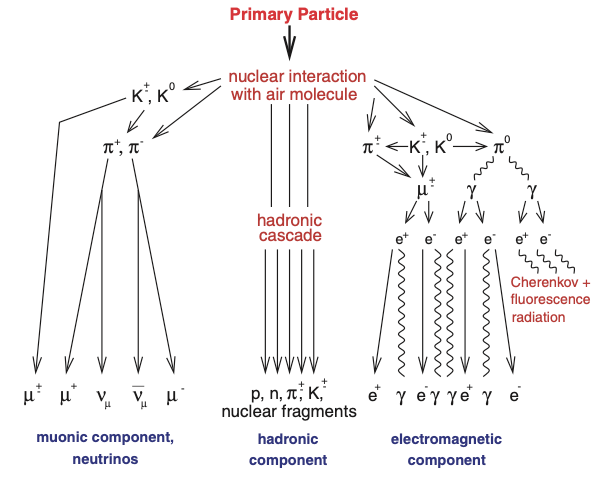
\includegraphics[scale=0.3]{Plots/Air shower illustration}
  \caption{Illustration of a hadronic air shower. It consists of an electromagnetic component (right), a hadronic component (middle) and the muonic component (left) which is central for this analysis. \cite{Haungs}}
  \label{fig:Air shower illustration}
\end{figure}
When cosmic rays interact with nuclei in the atmosphere they can produce particles who in turn decay or interact with the atmosphere again resulting in a cascade of particles called extensive air-shower. A hadronic shower is illustrated in Figure $\ref{fig:Air shower illustration}$.
The development of such events is described by the cascade equations which can only be solved numerically for example using MCEq \cite{gaisser2019precision}.
A number of different particles created in air showers can produce muons upon decay and thereby impact the atmospheric muon flux. 
Atmospheric muons are produced in hadronic cascades, so a large majority of the corresponding events are bundles of multiple muons instead of single muons futher complicating energy reconstructions. The number of muons in those bundles ranges over multiple orders of magnitude.
%Those interactions can produce Mesons and Baryons some of which in turn produce muons upon decay.
The biggest contribution to the muon flux is made by charged pions and kaons via the channels \cite{gaisser_engel_resconi_2016}:
\begin{align}
  \pi^{\pm} \rightarrow \mu^{\pm}+\nu_{\mu}(\bar{\nu}_{\mu}) (BR\approx100\%), \\
  K^{\pm} \rightarrow \mu^{\pm}+\nu_{\mu}(\bar{\nu}_{\mu}) (BR\approx63,6\%). 
\end{align}
Pions and kaons are the particles created at the highest rate in primary interactions leading to a high number of atmospheric muons being created. Other leptons like electrons can theoretically also be created in air showers but those decay modes of the $\pi^{\pm}$ and $K^{\pm}$ can be neglected because of their low branching ratio.
Muons stemming from $\pi^{\pm}$ and $K^{\pm}$ decay are called conventional muons. 

Calculating the flux of atmospheric muons is highly complex because decay, interaction and energy loss have to be accounted for.
There are also additional uncertainties involved because the production of charged pions and kaons depends on the primary cosmic ray spectrum which is not precisely known.
%Because atmospheric density varies with the zenith angle muons show an angular dependency of: $\frac{\sec\Theta}{E_{\mu}}$.

Aside from the conventional channels there are various other modes contributing to the muon flux the most important of those being the decay of charmed hadrons ($D^0$, $D^+$, $D_s^+$, $\Lambda_c$ as well as their antiparticles) and the decay of unflavored mesons ($\eta$, $\eta$', $\rho^0$, $\omega$, $\Phi$) into muon-antimuon-pairs \cite{Illana_2011}. Muons generated this way are called prompt.
Even though charmed mesons like the $D^{\pm}$ exhibit significant branching ratios in the relevant decay modes for example \cite{pdg}:
\begin{align}
  D^0 \rightarrow K^-\mu^+\nu_{\mu}(BR\approx5,3\%), \\
  D^{\pm} \rightarrow \bar{K}^0\mu^+\nu_{\mu}(BR\approx14,03\%).
\end{align}
The muons produced that way are the much smaller contribution to the atmospheric muon flux for almost all energies because the corresponding parent particles are produced in the primary hadronic interactions at a much lower rate than pions or kaons. 
In contrast to that the unflavored mesons have an energy spectrum that is similar to pions or kaons but their branching ratios to the modes including muons are very small.

As previously established prompt and conventional muons are distinguished by definition by their parent particles which in turn differ in their mean lifetime:
Pions and kaons have a lifetime of $\tau_{\pi^{\pm},K^{\pm}} \sim 10^{-8}\si{\second}$. In comparison to that charmed particles have a much lower lifetime of $\tau_{\mathrm{charmed}} \sim 10^{-12}-10^{-13} \si{\second}$ \cite{pdg}.
Following this pions and kaons usually interact rather than decay in a majority of cases while the parent particles of other contributions in most cases decay before having interacted hence their name: 'prompt'.
\begin{figure}
  \centering
  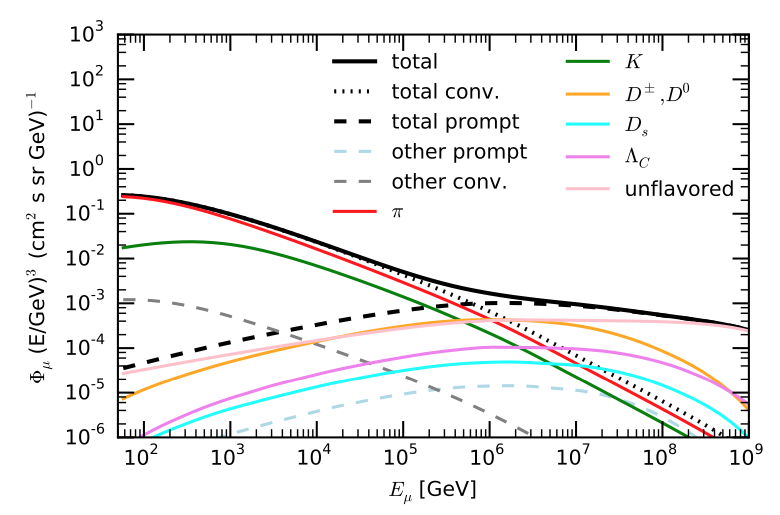
\includegraphics[scale=0.35]{Plots/Prompt vs conventional flux}
  \caption{The atmospheric neutrino flux divided into the different contributing factors based on numerical solutions of the Cascade equations. At about $E_{\mu}\approx 5*10^5\si{\giga\electronvolt}$ there is a threshold for the prompt component becoming the dominant. From $E_\mu=10^7\si{\giga\electronvolt}$ upwards the contribution of charmed particles falls of and the whole flux is dominated by the decay of unflavored mesons. Amongst the charmed particles the $D^{\pm,0}$ is the most relevant. \cite{fedynitch2015calculation}}
  \label{fig:Conventional vs prompt flux}
\end{figure}
Because of time dilatation the decay probability of the prompt component is additionally suppressed at high energies. Resulting from this effect two major differences between prompt and conventional component arise:
Conventional muons have a much steeper energy spectrum than their prompt counterpart, therefore the prompt component becomes dominant at high energies as illustrated in Figure $\ref{fig:Conventional vs prompt flux}$ \cite{fedynitch2015calculation} and the prompt component has an isotropic angular distribution while the spectrum of conventional muons contains the factor: $\sec \Theta / E_{\mu}$ relative to the primary cosmic ray spectrum depending on the zenith angle $\Theta$ \cite{gaisser_engel_resconi_2016}.
%The ladder can be explained with atmospheric density varying with the zenith angle impacting interactions.
Because the parent particles of prompt muons usually don't interact they are isotopically distributed.
\cite{Illana_2011} \cite{gaisser_engel_resconi_2016}
\section{The IceCube Neutrino Observatory}
The IceCube Neutrino Observatory is a kilometer-scale detector located in the South Pole ice.
When charged particles move through a medium faster than the speed of light in that medium the particle emits light in a cone with a characteristic opening angle along its track \cite{Mikkelsen_2016}. This so-called Cherenkov effect is the principle the IceCube detector is based on.

The essential elements of the detector are the digital optical modules (DOMs). They measure charge pulses using Photo-Multiplier-Tubes (PMTs) to detect the Cherenkov light emitted by charged particles (leptons) travelling the ice.
The original purpose of the Detector is to measure leptons generated when neutrinos interact with the ice. Atmospheric muons which are the focal point in this analysis are considered background for neutrino measurements.
\begin{figure}
  \centering
  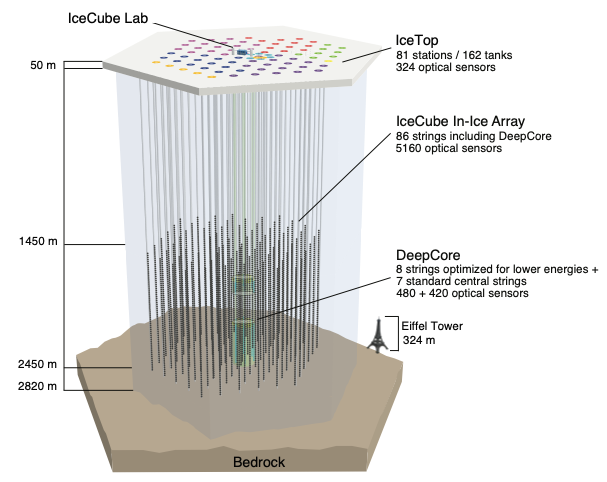
\includegraphics[scale=0.5]{Plots/IceCube schematic}
  \caption{Schematic picture of the IceCube Neutrino Observatory. \cite{Aartsen_2017}}
  \label{fig:IceCube schematic}
\end{figure}

A number of different arrays make up the detector the most import of those being the in-ice array made up of $5160$ DOMs deployed along $78$ vertical strings between depths of $\SI{1450}{\meter}$ and $\SI{2450}{\meter}$ covering a total area of $\SI{1}{\kilo\meter}^3$. 
The high detection volume is essential to detect neutrinos with a high sensitivity because of their low interaction probability. 
The strings are positioned in an approximate hexagonal grid ($\SI{125}{\meter}$ spacing) with each string containing $60$ DOMs and function to send the data collected by the DOMs to the surface via copper wires. All cable strings lead to the servers in the IceCube Laboratory (ICL) where the data is analyzed and distributed all over the world.
In addition to the main in-ice array the deep-core array composed of 8 strings optimized to register lower energy events.
Those strings are deployed in a tighter non-hexagonal configuration with a mean spacing of ($\SI{72}{\meter}$). The DeepCore array is divided into upper and lower DeepCore divided by a dust layer in the ice.
The whole IceCube Neutrino Observatory including the different sub-arrays is illustrated in Figure $\ref{fig:IceCube schematic}$.

The south-pole ice is especially suitable for the detection of Cherenkov light because it offers high quantities of interaction material for neutrinos as well as a high optical attenuation length \cite{Aartsen_2017}.
Those properties enable the detector to cover the large volume needed for the detection of neutrinos with a relatively high spacing of DOMs.  \cite{Aartsen_2017}
\section{Convolutional neural networks}
The fundamental basics of convolutional neural networks are mentioned at first.
Secondly, the specific CNN structure used in IceCube is stated.
\subsection{General theory on CNNs}
Neural Networks are digital structures designed to mimic the function of the human brain but when broken down they are just a highly complex optimization problem.
%\begin{figure}
%  \centering
%  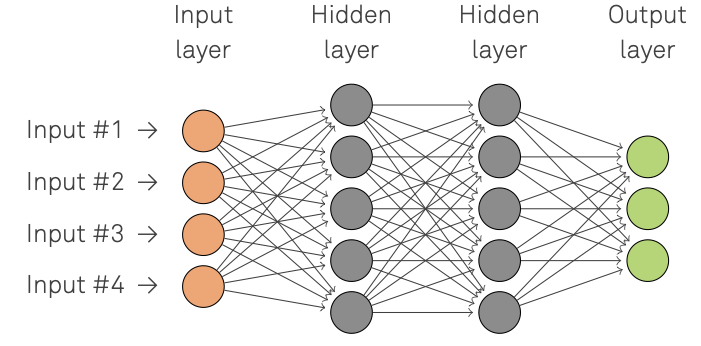
\includegraphics[scale=0.45]{Plots/Neural Network schematic}
%  \caption{Schematic of a neural network with two hidden layers.}
%  \label{fig:Neural Network schematic}
%\end{figure}
A Neural Network consists of an input and an output layer as well as one or multiple hidden layers in between whose output is not observed directly.% An example of such a network architecture can be seen in Figure $\ref{fig:Neural Network schematic}$. 
The output of each node is calculated as a linear combination of all outputs by the nodes in the previous layer. The parameters of the individual linear combinations linking the nodes are called weights. Additionally, a so-called activation function is applied to the computed linear combination of inputs to make the model nonlinear.
The activation function as well as number and size of the hidden layers have to be chosen based on the application. The fully connected part of the neural network used in this analysis is always identical and consists of one hidden layer with 50 nodes and the 'elu' activation function \cite{clevert2016fast}.
The network 'learns' those weights by optimizing a loss function designed to describe how well the regression (or classification) fits the truth.
This loss function is then iteratively minimized using complex numerical methods \cite{hastie2009elements}. The exact nature of the loss function and the optimization method are chosen based on the problem, in this case it is the 'Adam' optimizer \cite{kingma2017adam} in combination with a Gaussian-likelihood loss function.

For certain applications like image recognition it is sensible to use a special form of neural network called convolutional neural network.
This network architecture is aimed at utilizing translation invariance, the fundamental concept that the same physical process looks identical no matter where in the detector it happens.
To achieve this a filter of a certain shape unique to the dimensionality of the input data is applied locally weighting every node with the ones in its immediate surrounding.
This filter is applied equally to every node creating so-called feature maps who are than used by a fully connected network to make a prediction. In addition to that the process of pooling is used to reduce data dimensionality and is especially useful for problems with a high number of input variables like in the case of the IceCube detector.
Pooling describes the summarization of multiple data points in a subregion to only one value in most cases by taking the average or the maximum of the values in the designated field. By the application of such a pooling filter the size of the feature maps can be reduced significantly based on the filter size. \cite{dumoulin2018guide} 
\subsection{IceCube specific CNN}
To suit the unique hexagonal structure and data input format a network was designed specifically to analyze IceCube data \footnote{The neural network is available at:https://github.com/icecube/dnn\_reco}.
\begin{figure}
  \centering
  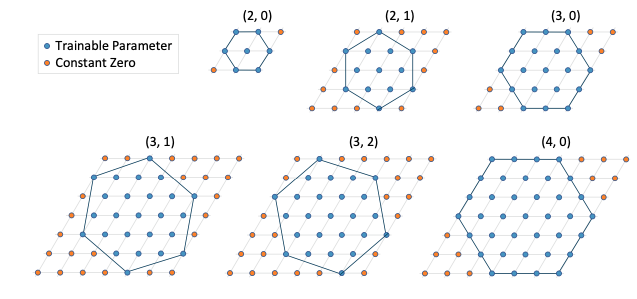
\includegraphics[scale=0.6]{Plots/Hexagonal Filters}
  \caption{Hexagonal convolutional Filters. Each Filter can be described by two parameters in the xy-plane: (size, orientation). All networks presented in this analysis have the shape (2,0,3) (top left) with the third number representing the convolution along the z-axis. \cite{Abbasi_2021}}
  \label{fig:Hexagonal Filters}
\end{figure}
To fit the architecture of IceCube the convolutional filters of the network are hexagonal shaped as illustrated in Figure $\ref{fig:Hexagonal Filters}$.
A problematic factor when looking at IceCube data is the data input format. IceCube DOMs measure the deposited charge depending on the time as a pulse series.
\begin{figure}
  \centering
  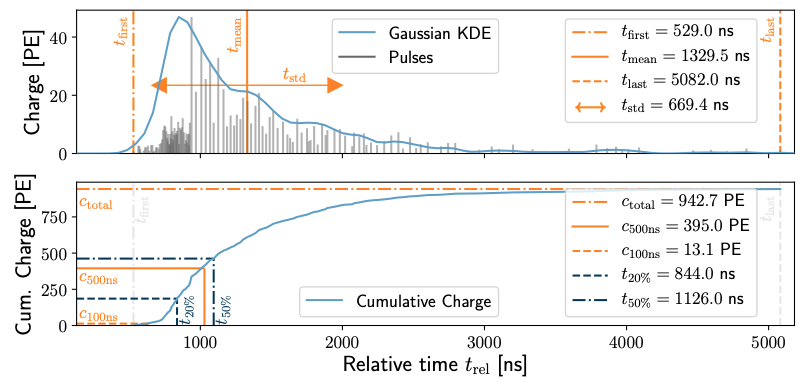
\includegraphics[scale=0.5]{Plots/Data input}
  \caption{Construction of the input features based on an IceCube pulse series (top) and the resulting cumulative charge (bottom). \cite{Abbasi_2021}}
  \label{fig:Data input}
\end{figure}
To achieve an input of constant size for every DOM and every event without making the model to complex each pulse series is broken down to a number of discrete input features. Figure $\ref{fig:Data input}$ shows a typical IceCube pulse series and the features generated from it. Of the nine input features the network was originally designed on only three are used here to hold runtimes low: The total charge $c_{\mathrm{total}}$, the relative time of the first pulse $t_{\mathrm{first}}$ and the standard deviation of pulse times $t_{\mathrm{std}}$.

Having generated the three input features they have to be transformed to ultimately be applicable to a CNN.
The hexagonal shaped data of the main array is transformed onto a rectangular grid by aligning the rows and padding the remaining points with zeros. Deep Core is too asymmetric to be put on a rectangular grid, so the corresponding data is aligned next to each other on a 2 dimensional grid.
Additionally, all charge and energy related features and labels are put on a logarithmic scale via the transformation:
\begin{equation}
  X'=\ln(1+X)
\end{equation}
to compensate for the big range those values cover. Then all values are centered around zero and normalized to unit variance:
\begin{equation}
  X''=\frac{X'-\bar{X'}}{\sigma_X+\epsilon}
\end{equation}
with a small constant $\epsilon=10^{-4}$ to avoid division by zero.
\cite{Abbasi_2021}
\chapter{Reconstruction performance}
In this chapter the performance of the reconstruction of the bundle and leading muon energy respectively by networks with different architectures is evaluated and compared to an alternative method not based on machine learning.
\section{Bundle energy}
The first reconstructed label is the energy of the muon bundle at detector entry.
Because this energy is strongly correlated to the energy deposited in the detector \cite{Aartsen_2014}, which in turn can be inferred from the total charge measured by the DOMs, it is expected that this is a value that can be reconstructed better compared to the energy of the leading muon.
%\subsection{Learning process}
\subsection{Correlation}
A neural network with eight convolutional layers and a kernel shape of $(2,0,3)$ and a network with a reduced number of convolutional layers result in reconstructions as displayed in $\ref{fig:Correlation 8L}$. 
\begin{figure}[h]
  \centering
  \begin{minipage}[t]{0.49\textwidth}
    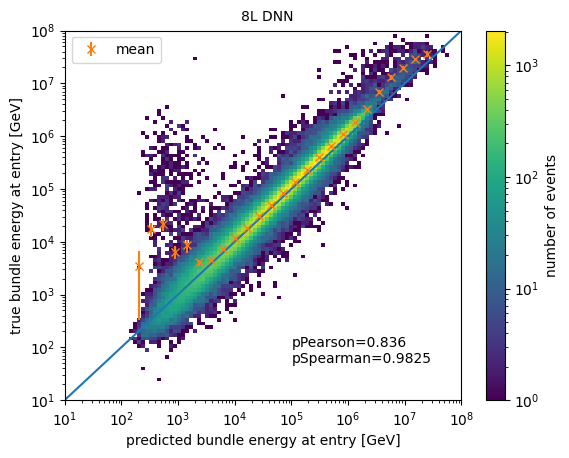
\includegraphics[width=\textwidth]{Plots/Correlation bundle energy std DNN (8L)}
  \end{minipage}
  \begin{minipage}[t]{0.49\textwidth}
    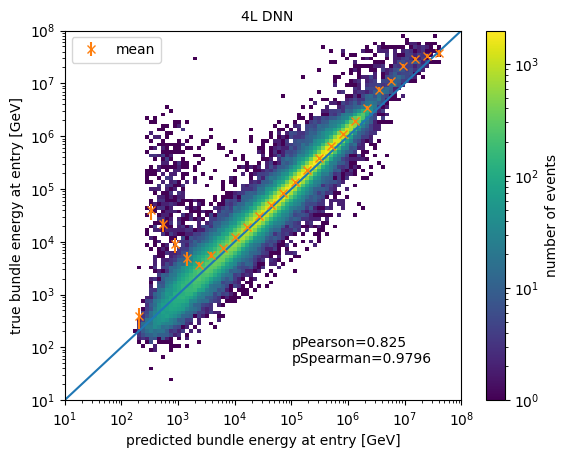
\includegraphics[width=\textwidth]{Plots/Correlation bundle energy small DNN (4L)}
  \end{minipage}  
  \caption{Correlation of the predicted and true bundle energy as an unweighted two-dimensional histogram for neural networks with four convolutional layers (4L,right) and eight convolutional layers (8L,left) on the main array. The strength of the linear and monotonic correlation between prediction and truth are indicated by Pearson and Spearman correlation coefficients respectively. In the low energy region the mean is dominated by outliers where the energy was significantly underestimated. In the high energy region there are fewer outliers, but the reconstruction is biased towards underestimation.}
  \label{fig:Correlation 8L}
\end{figure}
%\begin{figure}
%  \centering
%  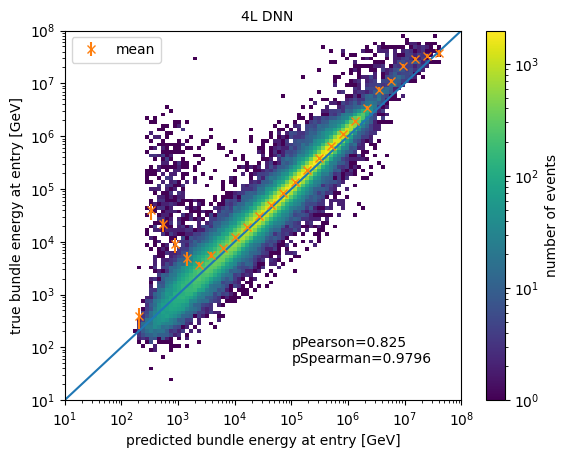
\includegraphics[scale=0.6]{Plots/Correlation bundle energy small DNN (4L)}
%  \caption{Correlation of the predicted and true bundle energy for a smaller Network with only four convolutional layers. The reduced network size does not result in changes significant enough to be seen with the naked eye, even though the linear and monotonic correlation is slightly reduced compared to the bigger network.}
%  \label{fig:Correlation 4L}
%\end{figure}

%A network with a reduced number of convolutional layers is shown in $\ref{fig:Correlation 4L}$.
Qualitatively both networks perform very similar with only minor improvements in linear correlation for the 8L version. 
The bias in the high energy region most likely is a result of the detector not being able to resolve all deposited energy leading to systematic underestimation.

To assess, if the application of a neural network for this reconstruction task makes sense, it is important to also look at standard reconstruction methods and their performance
in comparison to the DNN based approach. For this specific task it makes sense to use the MuEX reconstruction \cite{20.500.12030_2899} as a comparison despite the fact that far more 
precise methods exist, because those would not be applicable for prompt analysis due to their extremely high runtime.
\begin{figure}
  \centering
  \begin{minipage}[t]{0.49\textwidth}
    \includegraphics[width=\textwidth]{Plots/correlation_bundle_energy_muex}
  \end{minipage}
  \begin{minipage}[t]{0.49\textwidth}
    \includegraphics[width=\textwidth]{Plots/correlation_bundle_energy_muex2}
  \end{minipage}
  \caption{Correlation of the true and predicted bundle energy for the MUeX reconstruction. In the right plot, the x-axis is expanded to show the extreme outliers to unrealistically high energies. The monotonic correlation is weaker than that of both DNNs. The Pearson coefficient is not stable against the outliers, so it is less meaningful here.}
  \label{fig:Correlation MUeX}
\end{figure}
Figure $\ref{fig:Correlation MUeX}$ shows that aside from the generally higher spread the MuEX Fit especially shows a high number of outliers in the high energy region, where high energies up to $\SI{e28}{\giga\electronvolt}$ are estimated. 
As a consequence, in contrast to the DNN, the MuEX Fit is prone to overestimation for high energies.
This is a particularly problematic effect for the purpose of this analysis, because events with an energy over $\SI{100}{\giga\electronvolt}$, which are interesting for prompt analysis, are spread over more than $20$ orders of magnitude in the reconstruction likely leading to problems with identifying the prompt component.
Furthermore, the MuEX reconstruction does not provide information about the uncertainty of the reconstruction making it harder to cut out the unscientific values and reduce the Data to a subset of well reconstructed events.

Based on the uncertainty-reconstruction made by a separate subnetwork a cut can be made to filter for events estimated with a lower uncertainty. 
An uncertainty cut can be made on the absolute value given by the network because it is already made based on the transformed values.
The exact value to cut on has to be chosen depending on the application and how much loss of data is affordable. The Dataset used for evaluation only has a low number of events with high energies the cuts are additionally hard to evaluate. One point of reference is the Pearson correlation coefficient depending on the cut.
\begin{figure}
  \centering
  \begin{minipage}[t]{0.49\textwidth}
    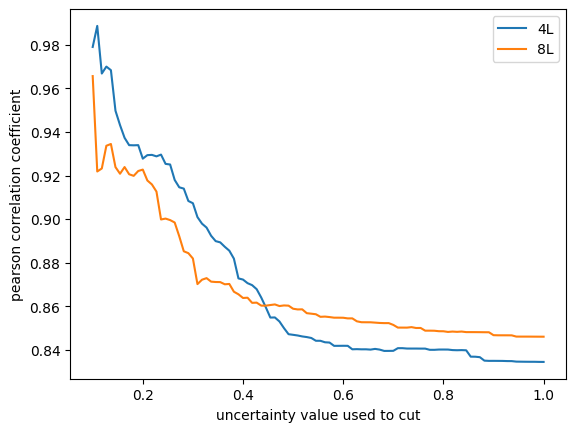
\includegraphics[width=\textwidth]{Plots/Pearson depending on cut}
  \end{minipage}
  \begin{minipage}[t]{0.49\textwidth}
    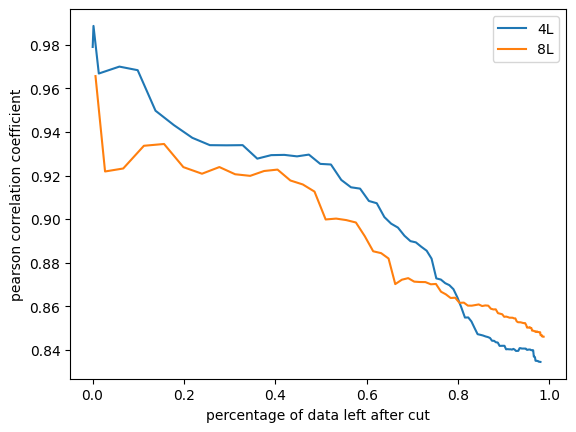
\includegraphics[width=\textwidth]{Plots/Pearson depending on cut percentage}
  \end{minipage}
  \caption{Pearson correlation coefficient depending on the chosen uncertainty cut (left) and depending on the percentage of data after the cut (right). In the left plot it is cut for all events smaller than or equal to the displayed logarithmic uncertainty.}
  \label{fig:Pearson(cut)}
\end{figure}
The impact of the different cuts on linear correlation is shown in Figure $\ref{fig:Pearson(cut)}$.
\begin{figure}[h]
  \centering
  \begin{minipage}[t]{0.49\textwidth}
    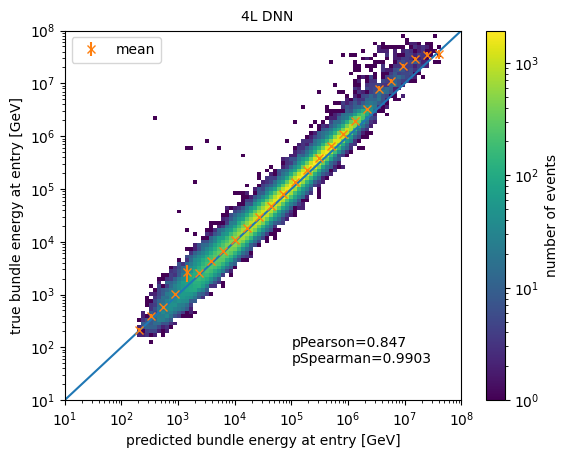
\includegraphics[width=\textwidth]{Plots/Correlation bundle energy (4L, cut)}
  \end{minipage}
  \begin{minipage}[t]{0.49\textwidth}
    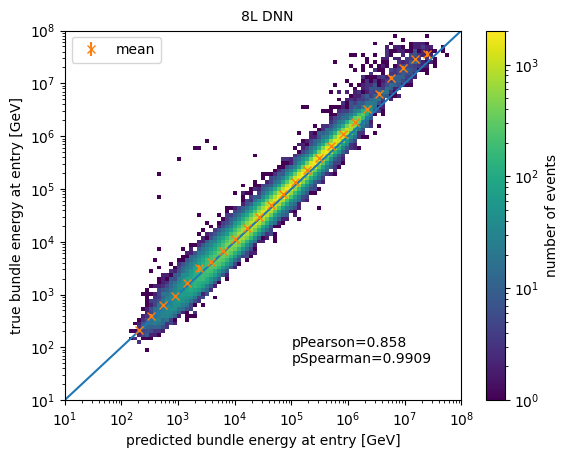
\includegraphics[width=\textwidth]{Plots/Correlation bundle energy (8L, cut)}
  \end{minipage}
  \caption{Correlation plot between reconstructed and true bundle energy for events with an estimated log-uncertainty smaller than $0.5$. Monotonic and especially linear correlation are significantly enhanced. While this removes the smearing effects seen in Figure $\ref{fig:Correlation 8L}$ for lower predicted energies the bias seen for high energies can not be corrected.}
  \label{fig:Correlation cut}
\end{figure}
As seen in Figure $\ref{fig:Correlation cut}$ making a quality cut especially eliminates events with small reconstructed energies, where significant smearing effects are seen when not making a cut.
The loss of prompt events is especially low, supporting the fact that the cut is actually suitable.
After the cut both networks show a linear correlation that is almost equal. The main advantage of the 8L model in this case is the increased amount of Data after the cut ($\SI{87.1}{\percent}$ compared to $\SI{84.9}{\percent}$ for the 4L DNN) because it generally estimates events with a high uncertainty less often.
\subsection{Energy spectrum}
With the energy reconstruction of the neural networks an energy spectrum can be generated, in this case using the weighting for the GaisserH3a-model \cite{gaisser2013cosmic}.
In this case only event rates are displayed. To generate an actual energy spectrum one would have to account for systematic effects of the detector such as the detector sensitivity as well as generate the energy on the surface based on the reconstructed energy at detector entry.
The resulting spectrum is analyzed in the high energy domain, where the prompt component is expected to be dominant.
\begin{figure}
  \centering
  \begin{minipage}[t]{0.49\textwidth}
    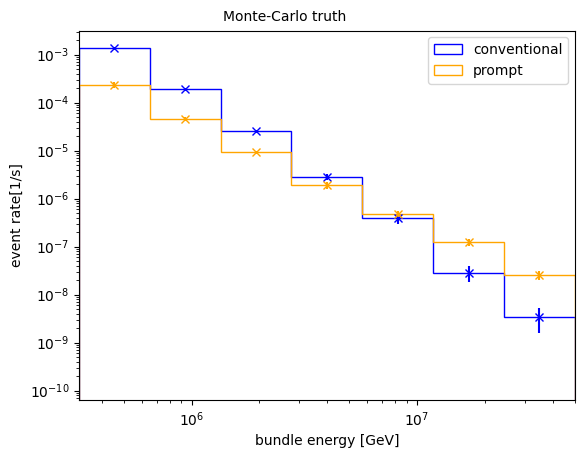
\includegraphics[width=\textwidth]{Plots/muon flux monte carlo bundle}
  \end{minipage}
  \begin{minipage}[t]{0.49\textwidth}
    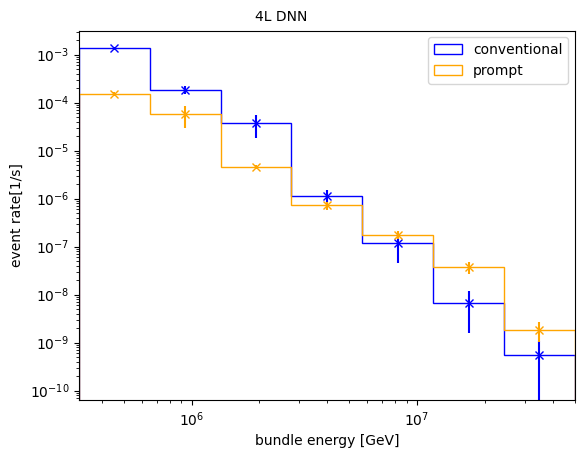
\includegraphics[width=\textwidth]{Plots/muon flux small dnn bundle}
  \end{minipage}
  \begin{minipage}[t]{0.49\textwidth}
    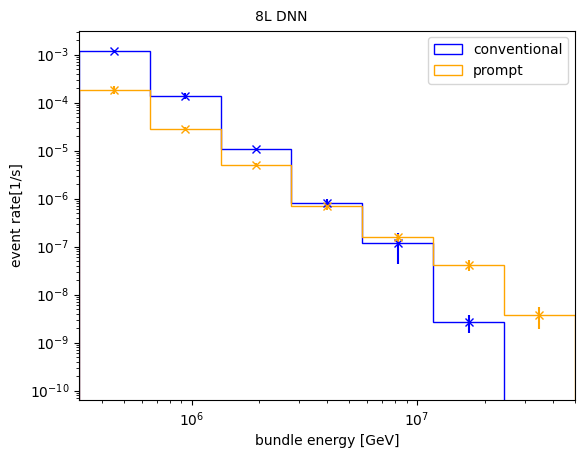
\includegraphics[width=\textwidth]{Plots/muon flux std dnn bundle}
  \end{minipage}
  \begin{minipage}[t]{0.49\textwidth}
    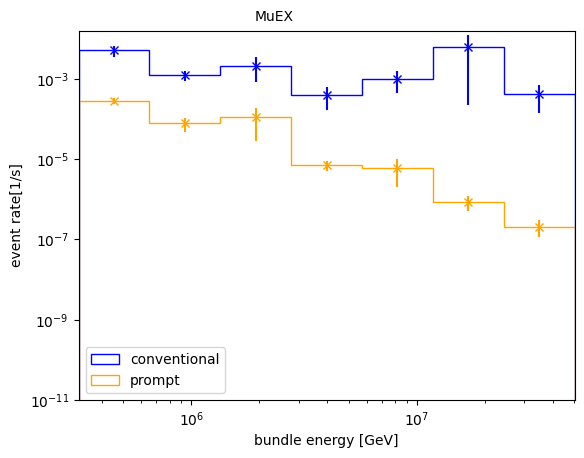
\includegraphics[width=\textwidth]{Plots/muon flux MuEX}
  \end{minipage}
  \caption{The energy spectrum for bundle energies between $\SI{3e5}{\giga\electronvolt}$ and $\SI{5e7}{\giga\electronvolt}$ according to the Monte-Carlo data, the 4L-DNN, the 8L-DNN and the MuEX Fit. All spectra are divided into a prompt and a conventional component based on the nature of the leading muon. For weighting the GaisserH3a-model is used. The errorbars are calculated according to the Poisson statistic. Both DNNs are capable of displaying a dominant prompt component as expected looking at the Monte-Carlo data and therefore are suitable for prompt analysis. In contrast, the MuEX fit does not reconstruct the bundle energy well enough to see the prompt component as dominant. It is also apparent, that as expected based on the correlation plots shown previously, the MUeX Fit strongly overestimates the event rate in the high energy domain.}
  \label{fig:Energy spectrum DNNs}
\end{figure}

The energy spectra displayed in Figure $\ref{fig:Energy spectrum DNNs}$ demonstrate that both DNNs predict the prompt component to be dominant for very high energies.
Resulting from this, the 3 highest energy bins in both reconstructions provide sensitivity for prompt muons, meaning that they are suitable for prompt analysis.
The only slight caveat is the reduced event rate in those bins compared to the Monte-Carlo truth 
most likely caused by the systematic underestimation mentioned in the previous section.
In contrast to that the reconstruction provided by the MuEX fit predicts a very flat energy spectrum that significantly overestimates both prompt and conventional event rate for high energies due to the smearing effects seen in Figure $\ref{fig:Correlation MUeX}$
As the MuEX fit is apparently not capable of seeing a dominant prompt component it does not provide sensitivity for prompt muons and is therefore not applicable for an analysis of the prompt component.
\begin{figure}
  \centering
  \begin{minipage}[t]{0.49\textwidth}
    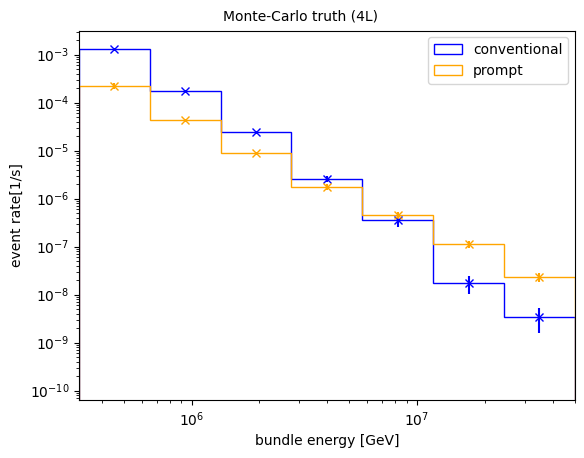
\includegraphics[width=\textwidth]{Plots/muon flux monte carlo bundle 4L cut}
  \end{minipage}
  \begin{minipage}[t]{0.49\textwidth}
    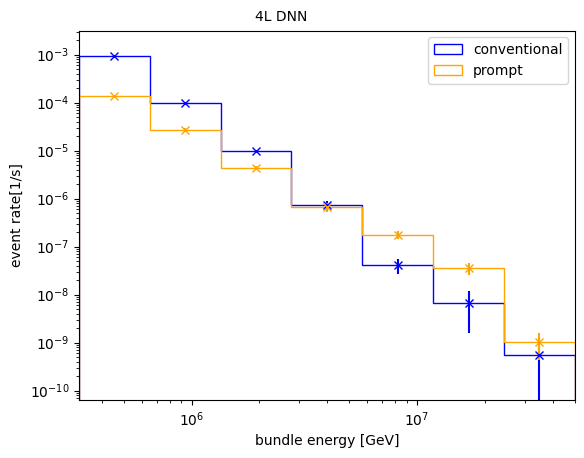
\includegraphics[width=\textwidth]{Plots/muon flux small dnn bundle cut}
  \end{minipage}
  \begin{minipage}[t]{0.49\textwidth}
    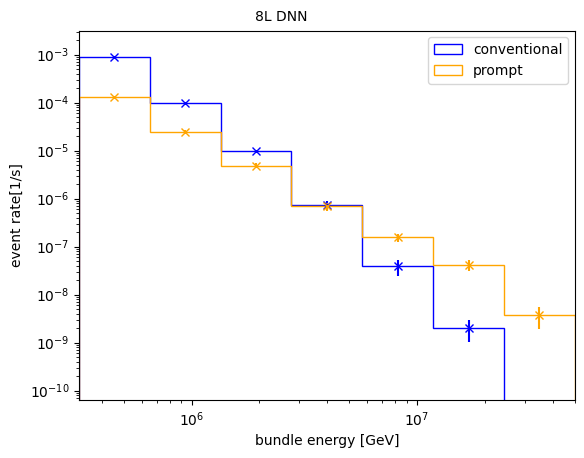
\includegraphics[width=\textwidth]{Plots/muon flux std dnn bundle cut}
  \end{minipage}
  \begin{minipage}[t]{0.49\textwidth}
    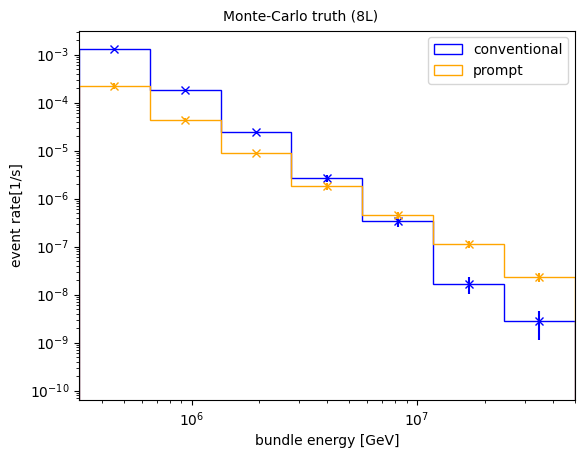
\includegraphics[width=\textwidth]{Plots/muon flux monte carlo bundle 8L cut}
  \end{minipage}
  \caption{Energy Spectrum of Monte-Carlo simulation and DNNs with the corresponding quality cuts. The cut is network specific so the Monte-Carlo truth has to be calculated for each network individually. Quality cuts on significantly lower uncertainties are hard to evaluate based on this dataset because of the low amount of data in the high energy region.}
  \label{fig:Energy spectrum DNNs cut}
\end{figure}

The spectrum of both networks after the application of the previously shown quality cuts is displayed in Figure $\ref{fig:Energy spectrum DNNs cut}$.
While the reconstruction still shows a sensitivity for the prompt component it is not a very significant improvement upon the raw reconstruction because the bias of the network is still present and therefore event rates in the relevant bins are still underestimated compared to the truth.
The more noticeable positive effects of the cut are in relevant energies lower than those considered in the spectra displayed here.
Another important factor to consider when comparing raw and cut Monte-Carlo is that the reduced amount of data results in increased Poisson-uncertainties. 
This effect is enhanced by the generally small statistic for energies above $\SI{1}{\peta\electronvolt}$.
This suggests that the size of the data set is not adequate to properly evaluate the neural network with the uncertainty cut applied from a certain threshold of data loss onwards because the Poisson-uncertainty in the prompt sensitive bins becomes to high to make sensible interpretations of the networks' performance.
The bigger network allows more events to pass the same uncertainty cut so it offers more statistic.

\section{Energy of the leading muon}
Reconstructing the energy of the most energetic muon in the shower is a much more challenging task for a neural network than just reconstructing the energy of the whole muon bundle because it does not suffice to sum up the deposited charge and conclude an energy. 
Additionally, there has to be an understanding of how dominant the leading muon is within the bundle.
In theory, this should be possible by considering the stochacisity of the deposited energy.
The basic idea behind this is that bundles where the energy is very equally distributed deposit energy more regularly than bundles with a dominant leading muon, who deposit energy large amounts of energy in singular spots.
How well the network can utilize this effect based only on the three input features is a main influence on the resulting reconstruction.
\subsection{Correlation}
\begin{figure}
  \centering
  \begin{minipage}[t]{0.49\textwidth}
    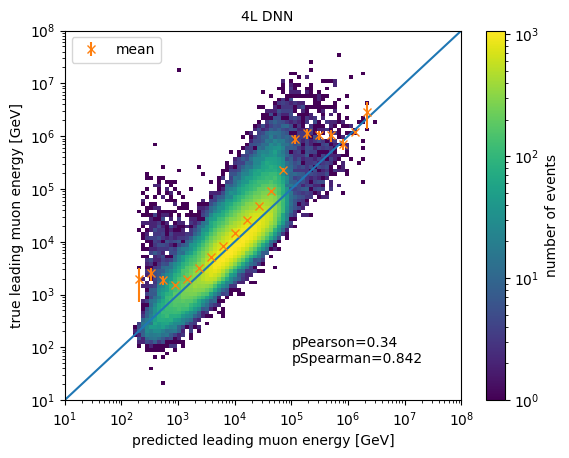
\includegraphics[width=\textwidth]{Plots/Correlation leading muon energy small DNN (4L)}
  \end{minipage}
  \begin{minipage}[t]{0.49\textwidth}
    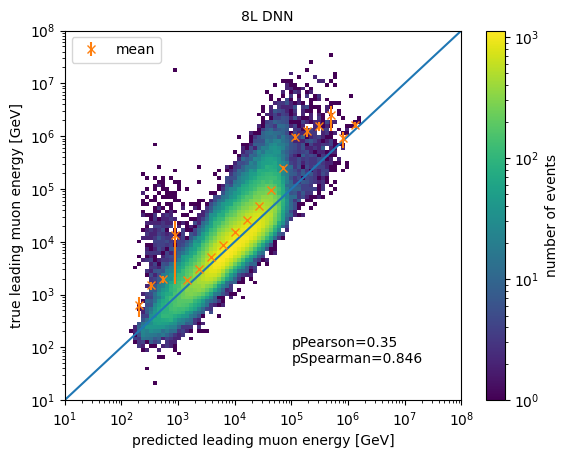
\includegraphics[width=\textwidth]{Plots/Correlation leading muon energy std DNN (8L)}
  \end{minipage}
  \caption{Correlation of true and reconstructed energy of the leading muon for the 4L and the 8L-DNN. Linear and monotonic correlation are reduced compared to the bundle energy. The mean of the true deposited energy is calculated in every third predicted energy bin. In some bins large outliers or low statistic result in high errors.}
  \label{fig:Correlation entry}
\end{figure}
The neural networks produce correlation plots as seen in Figure $\ref{fig:Correlation entry}$.
As expected, the correlation in general and the linear correlation in specific are weaker than that of true and reconstructed bundle energy for both networks.
In the predicted low energy region between $\SI{100}{\giga\electronvolt}$ and $\SI{10}{\tera\electronvolt}$ there are smearing effects similar to those seen for the bundle energy.
This suggests, that a bad reconstruction of the bundle energy in general also impacts the reconstruction of the leading muon energy.
In addition to that the mean shows strong underestimation from energies of $\SI{50}{\tera\electronvolt}$ upwards.
Especially obvious is, that both networks very rarely predict energies above $\SI{100}{\tera\electronvolt}$. The 4L-DNN for example only predicts $\SI{8.9}{\percent}$ of the events with a true leading muon energy over $\SI{100}{\tera\electronvolt}$ to be in that energy region.
This results in a large majority of the events expected in this region, where the prompt component is visible in theory, migrating to lower energy bins.
This soft threshold in the predicted energy is very problematic as seen in the energy spectrum in Figure $\ref{fig:Spectrum entry}$ because it almost completely eliminates the most important part of the spectrum from the prediction.

Resulting from this an uncertainty based cut on the data would not be sensible because the amount of data above $\SI{100}{\tera\electronvolt}$ is already massively reduced. It also appears that the events in that region are generally predicted with a high uncertainty so that they are eliminated at a much higher rate than other events.
\subsection{Energy spectrum}
\begin{figure}
  \centering
  \begin{minipage}[t]{0.32\textwidth}
    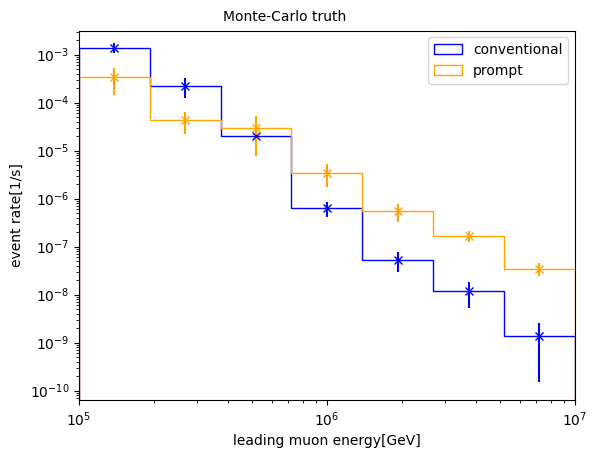
\includegraphics[width=\textwidth]{Plots/muon flux monte carlo entry}
  \end{minipage}
  \begin{minipage}[t]{0.32\textwidth}
    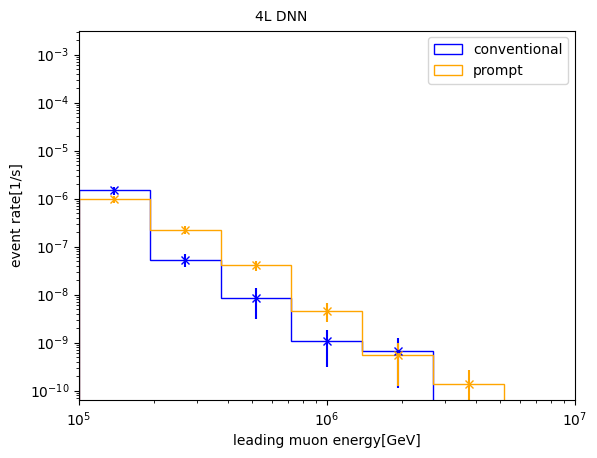
\includegraphics[width=\textwidth]{Plots/muon flux small dnn entry}
  \end{minipage}
  \begin{minipage}[t]{0.32\textwidth}
    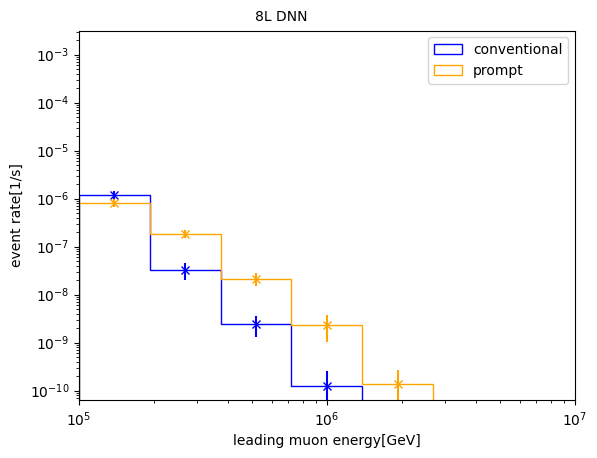
\includegraphics[width=\textwidth]{Plots/muon flux std dnn entry}
  \end{minipage}
  \caption{Simulated and reconstructed spectra for the 4L model (middle) and 8L model (right) of the leading muon weighted with the GaisserH3a-model are shown. The event rate of both components is underestimated by at least three orders of magnitude by both DNNs compared to the simulation even in the lowest energy bin. Moreover, the reconstructed spectra fall of steeper than they theoretically do. Even though both reconstructed spectra offer a sensitivity to the prompt component, the overall quality of the reconstruction does not suffice especially compared to the bundle energy.}
  \label{fig:Spectrum entry}
\end{figure}
Looking at the energy spectra of the leading muon in Figure $\ref{fig:Spectrum entry}$ it is apparent, that the systematic underestimation of high energetic muons and subsequent pileup of events in the lower energy-bins leads to reduced event rates in the reconstruction.
Resulting from this the reconstruction of the leading muon energy is not sensible to use compared to the bundle energy, although the leading muon energy provide theoretically better information on the prompt component as demonstrated in the Monte-Carlo spectrum in Figure $\ref{fig:Spectrum entry}$.
\subsection{Leading fraction}
The leading fraction is defined as the fraction of the bundle energy carried by the leading muon: $f_{\mathrm{lead}}=\frac{E_{\mathrm{lead}}}{E_{\mathrm{bundle}}}$.
As it is the essential difference between leading muon energy and the bundle energy the leading fraction was explicitly estimated by the networks as a separate label.

One way to further evaluate the reconstruction of the leading muon energy is to check for the impact of the leading fraction on the predicted leading muon energy.
Based on the assumption, that more dominant leading muons should be easier to identify within the bundle and therefore be reconstructed more precisely, a cut is performed for events in which the leading muon carries a high percentage of the bundle energy, in this case more than $15\%$.
\begin{figure}
  \centering
  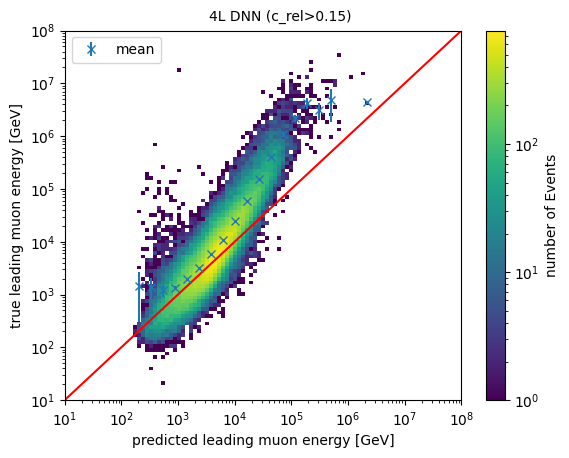
\includegraphics[scale=0.6]{Plots/Correlation leading muon energy smal dnn (c_rel>0.15)}
  \caption{Predicted and true energy of the leading muons for all events satisfying the condition: $f_{\mathrm{lead}}>0.15$. There is a significant bias to underestimation increasing with the predicted energy. The well reconstructed events in the high energy region are almost completely removed by the cut.}
  \label{fig:Correlation entry cut}
\end{figure}
The resulting correlation displayed in Figure $\ref{fig:Correlation entry cut}$ demonstrates that the assumption does not hold true.
Instead, the cut results in a bias increasing with the predicted energy.
Apparently the events with a high leading fraction are exactly those, who are underestimated for high energies by the networks.
\begin{figure}
  \centering
  \begin{minipage}[t]{0.32\textwidth}
    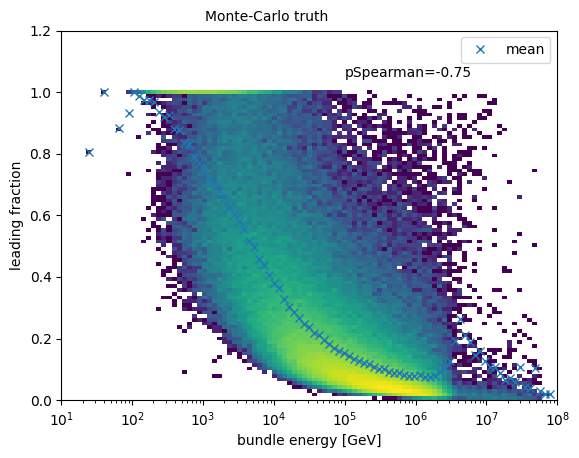
\includegraphics[width=\textwidth]{Plots/energy leading fraction correaltion monte carlo}
  \end{minipage}
  \begin{minipage}[t]{0.32\textwidth}
    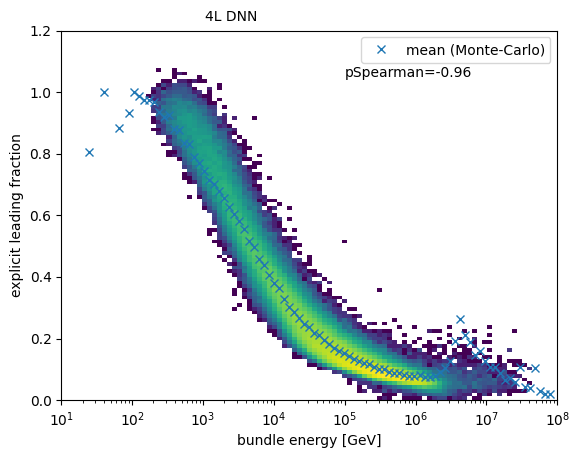
\includegraphics[width=\textwidth]{Plots/energy leading fraction correaltion small dnn explicit}
  \end{minipage}
  \begin{minipage}[t]{0.32\textwidth}
    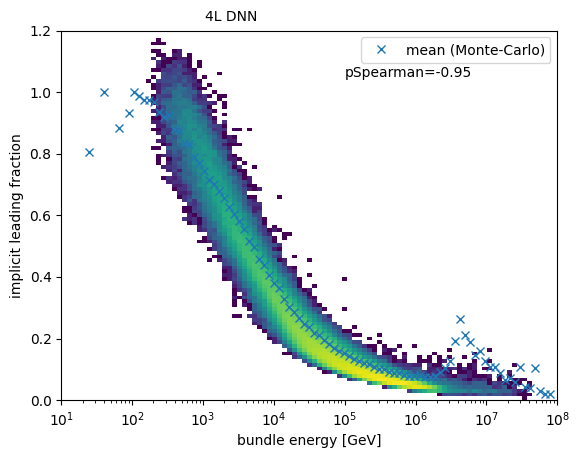
\includegraphics[width=\textwidth]{Plots/energy leading fraction correaltion small dnn implicit}
  \end{minipage}
  \caption{Correlation between bundle energy and leading fraction based on the Monte-Carlo data and the 4L-DNN. The implicit leading fraction in the right plot is calculated from predicted bundle energy and leading muon energy. The explicit leading fraction in the middle plot is predicted as a separate label by the network. The blue marks are identical in all three plots and represent the mean of the leading fraction in the bundle energy bins based on the simulation.}
  \label{fig:Correlation bundle leading}
\end{figure}

To further investigate the reasons for this phenomenon the relationship between bundle energy and leading fraction ($\ref{fig:Correlation bundle leading}$) is studied.
The Monte-Carlo simulation shows that while there is a general correlation between those two labels because it is less likely for high bundle energies to be dominated by the leading muon, this correlation is not strong ($\rho_{\mathrm{Pearson,MC}}=-0.75$).
In contrast to this the leading fractions estimated by the network are correlated stronger to the estimated bundle energy than they are based on the simulation with Pearson coefficients of $\rho_{\mathrm{Pearson,im}}=-0.95$ for the implicit and $\rho_{\mathrm{Pearson,ex}}=-0.96$ for the explicit leading fraction.
The maximum of both DNN based deviations is noticeably centered around the mean of the Monte-Carlo.
This suggests that the network does not estimate how dominant the leading muon is by using information on the stochasticity of the energy loss as was intended but instead learned to build an energy based mean using the reconstructed bundle energy.
In the context of prompt analysis the assumption that a high energetic bundle always has a very subdominant leading muon is problematic, because it automatically excludes the network from estimating a high energy above $\SI{100}{\tera\electronvolt}$ for the leading muon. Instead, it leads to the systematic underestimation of events with a high leading fraction (Figure $\ref{fig:Correlation entry cut}$) and the migration of high energetic events to lower energy bins in the prediction (Figure $\ref{fig:Correlation entry}$).
Considering that the explicit leading fraction is slightly less restricted for high energies than the implicit leading fraction there is the possibility that at least small improvements on the results can be made by using the explicit leading fraction to calculate the energy of the leading muon.
\section{Optimization}
Based on these results efforts can be made to try and improve the reconstruction of the energy of the leading muon and the bundle energy by changing the network's architecture.
\begin{figure}
  \centering
  \begin{minipage}[t]{0.49\textwidth}
    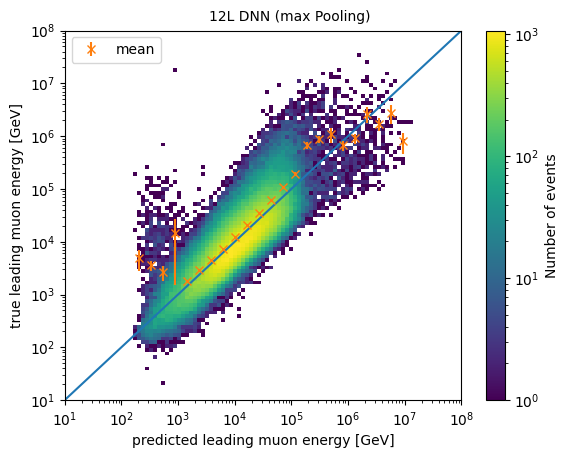
\includegraphics[width=\textwidth]{Plots/Correlation leading 12L max}
  \end{minipage}
  \begin{minipage}[t]{0.49\textwidth}
    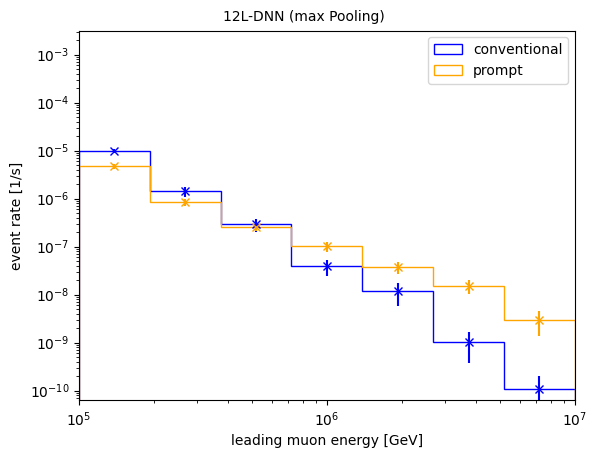
\includegraphics[width=\textwidth]{Plots/muon flux calculated 12L max}
  \end{minipage}
  \caption{Correlation plot and energy spectrum for a 12L network. The energy of the leading muon is calculated from the predicted leading fraction and bundle energy instead of being directly estimated. Improvements in linear and monotonic correlation are small, but the resulting spectrum shows significant improvements compared to previous models.}
  \label{fig:Correlation spectrum improved}
\end{figure}
By increasing the network size to 12 layers, increasing the number of filters and switching from average to max pooling as well as calculating the leading muon energy from the bundle energy and the explicit leading fraction a significantly improved reconstructed energy spectrum can be reached (Figure $\ref{fig:Correlation spectrum improved}$).
Those improvements are not visible in the Pearson or Spearman coefficients and even shows a lower Pearson coefficient, but the mean indicates less underestimation for high energies than the other models.
The most impactful change inferred from this is the increased amount of statistic above the critical $\SI{100}{\tera\electronvolt}$ threshold with almost $\SI{22.3}{\percent}$ of events actually in that region predicted to be in that region compared to $\SI{8.9}{\percent}$ for the 4L version using the direct approach for the leading muon energy.
\begin{figure}
  \centering
  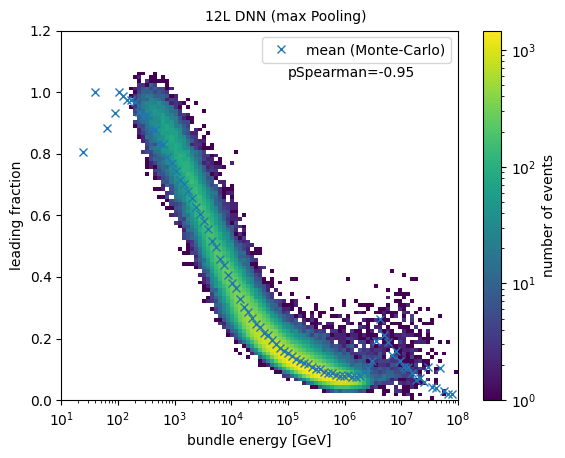
\includegraphics[scale=0.6]{Plots/Correlation bundle leading 12L}
  \caption{Correlation between bundle energy and leading fraction for the 12L-DNN with the mean of the corresponding plot done on the Monte-Carlo simulation.}
  \label{fig:Correlation bundle leading 12L}
\end{figure}
Although this new model offers strong improvements over the other reconstructions especially in terms of the energy spectrum generally and the prompt sensitivity specifically the Results still deviate from the simulated truth by one or two orders of magnitude and is not competitive compared to the reconstruction of the bundle energy.
Another look at the correlation of bundle energy and leading fraction (Figure $\ref{fig:Correlation bundle leading 12L}$) shows that even when making changes such as increasing the model size, the underlying problem remains the same.
As long as the prediction is made solely based on a correlation between bundle energy and leading fraction to an extent made up by the DNN the potential quality of the reconstruction is limited.
To find out, if there is a chance to get a higher quality reconstruction the networks' prediction of the leading muon energy first has to be separated from the predicted bundle energy.

In contrast to the prediction of the leading muon energy the bundle energy is already reconstructed well even for small models. The only significant point causing problems in this reconstruction is the bias to underestimation in the high energy region which is most likely a systematic problem that will not be fixed by increasing network size, so it makes more sense to try improving the smaller network.
The easiest way to make an improvement here is to switch from average to max pooling.
\begin{figure}
  \centering
  \begin{minipage}[t]{0.49\textwidth}
    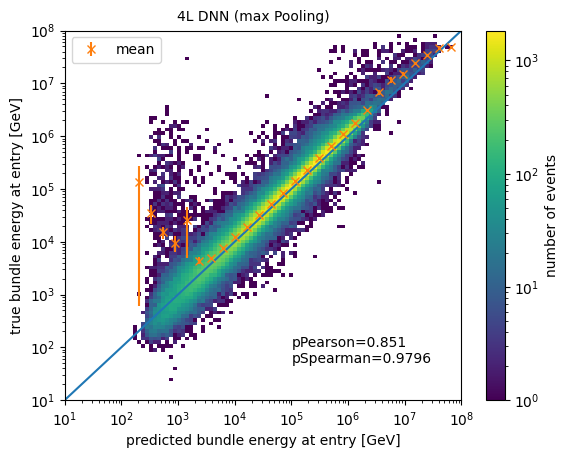
\includegraphics[width=\textwidth]{Plots/Correlation bundle 4L max}
  \end{minipage}
  \begin{minipage}[t]{0.49\textwidth}
    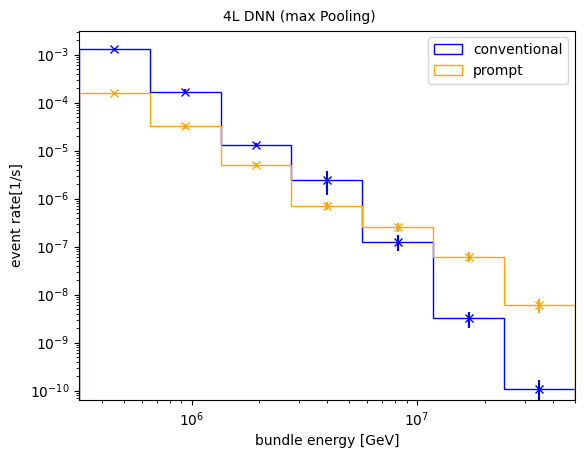
\includegraphics[width=\textwidth]{Plots/muon flux 4L max}
  \end{minipage}
  \caption{Correlation plot (left) and energy spectrum (right) of a 4L DNN using max instead of average pooling. Compared to the version of the same network using average pooling (Figures $\ref{fig:Correlation 8L},\ref{fig:Energy spectrum DNNs}$) it has a higher Pearson coefficient and better sensitivity for the prompt component especially under the consideration of uncertainties.}
  \label{fig:4L max}
\end{figure}
As seen in Figure $\ref{fig:4L max}$ the resulting network outperforms the 4L DNN with average pooling and even the 8L DNN when it comes to the linear correlation (Figure $\ref{fig:Correlation 8L}$) and also displays the better high energy spectrum when it comes to prompt sensitivity.

Another logical step is to use a single-label reconstruction for the bundle energy because previous results have shown, that the energy of the leading muon is at least currently not suitable for a prompt analysis. So utilizing the improvements offered by focusing the network on a single label has no significant disadvantages in this scenario. 
%\subsection{Differences between single- and multilabel regression}
%So far all neural networks presented in this thesis completed a multilabel regression task, meaning one network was trained to simultaneously reconstruct three different labels. In such a task problems can occur, because the different labels might differentiate massively in terms of how easy they are to learn for a network. This can lead to the loss function being dominated by one label and thus hindering the learning process of the others.
%It was demonstrated so far in this analysis, that the bundle energy is far easier to learn than the energy of the leading muon leaving room for problems in a multilabel regression.
%\begin{figure}
%  \centering
%  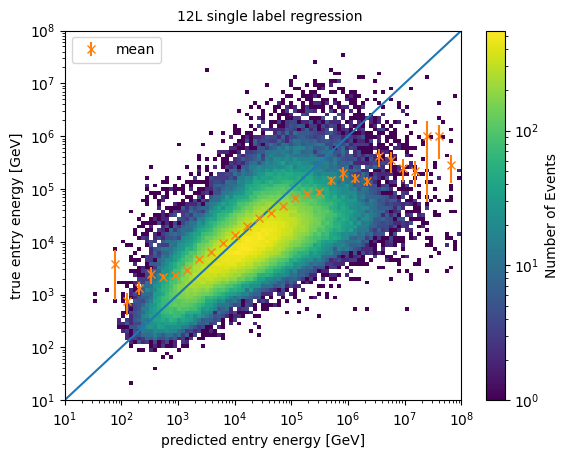
\includegraphics[scale=0.6]{Plots/Correlation 12L leading only}
%  \caption{}
%  \label{fig:Correlation 12L leading only}
%\end{figure}

%To examine, if the network is impacted in a problematic by the different impacts of the labels on the loss function two new networks were trained: One with a sole focus on the reconstruction of the bundle energy and one for the leading muon energy and the leading fraction.% The resulting reconstruction of the leading muon energy displayed in $\ref{fig:Correlation 12L leading only}$ strongly differs from the models trained on multilabel regression.
%Instead of underestimating in this case overestimation is dominant for high energies. While this is not necessarily a 'better' reconstruction it definitely the network almost definitely shows differences to previous tries going beyond getting better or worse at the fundamentally same method (in this case using the bundle energy as a proxy).
%An interesting change observed when taking the bundle energy out of reconstructions is an increased proneness to overtraining in the remaining labels. When trying to train a network only for the leading fraction the learning curve ($\ref{}$)
\chapter{Runtime comparison}
An important point to consider when evaluating the performance of the networks additionally to the quality of the reconstruction is the runtime.
Because atmospheric muons are created and detected at an extremely high rate the reconstructions applied to those events have to have a correspondingly low runtime.
\begin{figure}[h]
  \centering
  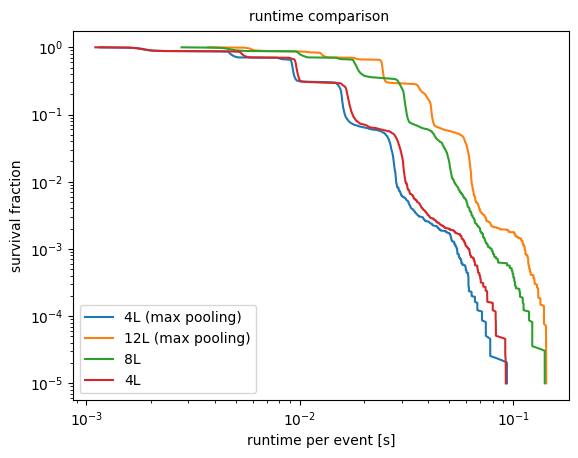
\includegraphics[scale=0.6]{Plots/Runtime comparison}
  \caption{Displayed on the y-axis is the fraction of events exceeding the runtime on the x-axis. As expected runtime generally increases with model complexity. Per event runtimes are given in reference to the time it takes the network to make a prediction. For the absolute runtime the preprocessing in the form of data transformation has to be considered. When comparing both networks this is unnecessary because the time it takes to preprocess does not depend on the network architecture.}
  \label{fig:Runtime comparison}
\end{figure}
The runtime performance of both networks is shown in the form of survival fractions in Figure $\ref{fig:Runtime comparison}$.
The 4L network has a median prediction time of $\mathrm{median}(t_{\mathrm{pred,4L}})=\SI{0.0096}{\second}$ which is almost twice as fast as the median of the 8L network ($\mathrm{median}(t_{\mathrm{pred,8L}})=\SI{0.0185}{\second}$) which in turn is faster than the median of the 12L network $\mathrm{median}(t_{\mathrm{pred,4L}})=\SI{0.0247}{\second}$.
A similar result is obtained by looking at the ratio of the runtimes of the DNNs. The median of the ratio $\mathrm{median}\left(\frac{t_{\mathrm{pred,8L}}}{t_{\mathrm{pred,4L}}}=\num{1.88}\right)$ indicates that the 4L DNN is almost twice as fast at making a prediction.
Although there also are instances in which the 8L-DNN is faster, those only make up $\SI{0.1}{percent}$ of all events.

A more interesting result is the deviating runtime between the 4L model running average pooling and 4L model running max pooling. Both models are otherwise not exactly identical because the model using max pooling has less convolutional layers in the lower DeepCore array, but the effects of this change are very small. Even though both networks share the same architecture aside from the pooling method Figure $\ref{fig:Runtime comparison}$ suggests that the network using max pooling is faster.
This is supported by the median runtime of $\mathrm{median}(t_{\mathrm{pred,4Lmax}})=\SI{0.0096}{\second}$. The benefit in runtime is only small with a ratio of $\mathrm{median}\left(\frac{t_{\mathrm{pred,4L}}}{t_{\mathrm{pred,4Lmax}}}\right)=\num{1.057}$ indicating a runtime improvement of over $\SI{5}{\percent}$ achieved by using max pooling.
But considering this as well as fact that the version using max pooling is faster for $\SI{90.9}{\percent}$ of all events it further supports the results obtained in the previous chapter suggesting that at least for a small network max pooling is the better option because it is both faster and delivers better reconstruction results.

\chapter{Conclusion and outlook}
The energy reconstruction of muons using machine learning methods shows differing results with respect to the application in a potential analysis of the prompt component of the atmospheric muon flux depending on what specifically is reconstructed.

Promising results are obtained for the reconstruction of the bundle energy, which can be estimated well enough even by a relatively small neural network to distinct the prompt component as the dominant contribution in the high energy domain as demonstrated in Figure $\ref{fig:Energy spectrum DNNs}$. 
The study of the non machine learning method MuEX shows worse reconstructions, which makes it impossible to detect the prompt component as shown in Figure $\ref{fig:Energy spectrum DNNs}$.
Depending on the runtime requirements, a network architecture with an increased number of convolutional layers can be used to achieve slight improvements as seen in Figures $\ref{fig:Correlation 8L}$ and $\ref{fig:Correlation spectrum improved}$ but considering the increase in runtime visible in Figure $\ref{fig:Runtime comparison}$ a smaller alternative is the better option in most cases.
With a median runtime of $\SI{0.0092}{\second}$ the 4L DNN with max pooling is twice as fast as the 8L network with a median runtime of $\SI{0.0185}{\second}$ and still shows comparable reconstruction results. 

In contrast to that the reconstruction of the energy of the leading muon proves to be more difficult. 
While it theoretically provides the better sensitivity for a prompt analysis this effect is completely negated by the reconstruction-quality. The energy reconstruczion of the leading muon is not competitive compared to the more reliable bundle energy reconstructions. This can bee seen in Figure $\ref{fig:Spectrum entry}$ and $\ref{fig:Correlation entry}$.
This discrepancy can be traced back to the strong correlation between bundle energy and leading fraction assumed by the network and displayed in $\ref{fig:Correlation bundle leading}$ leading it to avoid extreme values.
There are roughly three possible reasons for this phenomenon: The input features do not provide enough information to make assumptions about the stochasticity of the energy loss, the stochasticity seen by the DNN does not provide sufficient information about the dominance of the leading muon within the bundle or the stochasticity is not properly used to make a prediction by the network.
Whether there is no way to find a better mode of action provided only the three input features used here or whether it was not found by these specific network architectures can not be ultimately concluded.

To investigate the first two possible reasons it is necessary to create a dataset providing a separate label for the stochasticity.
Another network can be trained to predict this label, so it can be evaluated, if the stochasticity can be sufficiently estimated.
This procedure also enables an evaluation of the assumed correlation between the stochasticity and the leading fraction.
If the prediction of the stochasticity performs well, the estimation of the leading muon energy can be improved by changing the network architecture to use the provided information more efficiently.
Such optimizations can be performed by a hyperparameter optimization.
Possible improvements in performance can be reached by increasing the number of input features to increase the amount of information the network can utilize. Of nine possible features only three are used for this analysis. Additional charge related features like the charge collected in the first $\SI{100}{\nano\second}$ and $\SI{500}{\nano\second}$ respectively can improve information about the energy loss.
All in all, several networks have been studied and presented to estimate the muon bundle and leading muon energy sufficiently to provide a fast and accurate energy reconstruction to measure the prompt component of the atmospheric muon flux.
\appendix
% Hier beginnt der Anhang, nummeriert in lateinischen Buchstaben

\backmatter
\printbibliography
\chapter*{Danksagung}
Ich möchte mich zum Schluss in allen Bedanken, die mir den Abschluss dieser Arbeit ermöglicht haben.
Besonderer Dank gilt Herrn Prof. Dr. Dr. Wolfgang Rhode sowie Herrn Prof Dr. Carsten Westphal.
Weiterhin möchte mich speziell bei Pascal und Mirco für die ausführliche Betreuung meiner Arbeit sowie bei Lucas, Ludwig und Jean-Marco für ihre große Hilfsbereitschaft bedanken.
Auch bei den weiteren Mitgliedern der Arbeitsgruppe bedanke ich mich für zahlreiche interessante Gespräche und Diskussionen.

Zuletzt möchte ich mich bei meiner Familie für ihre Unterstützung bedanken, ohne die diese Arbeit nie möglich gewesen wäre.

\cleardoublepage
% From https://www.tu-dortmund.de/studierende/im-studium/pruefungsangelegenheiten/allgemeine-vordrucke/
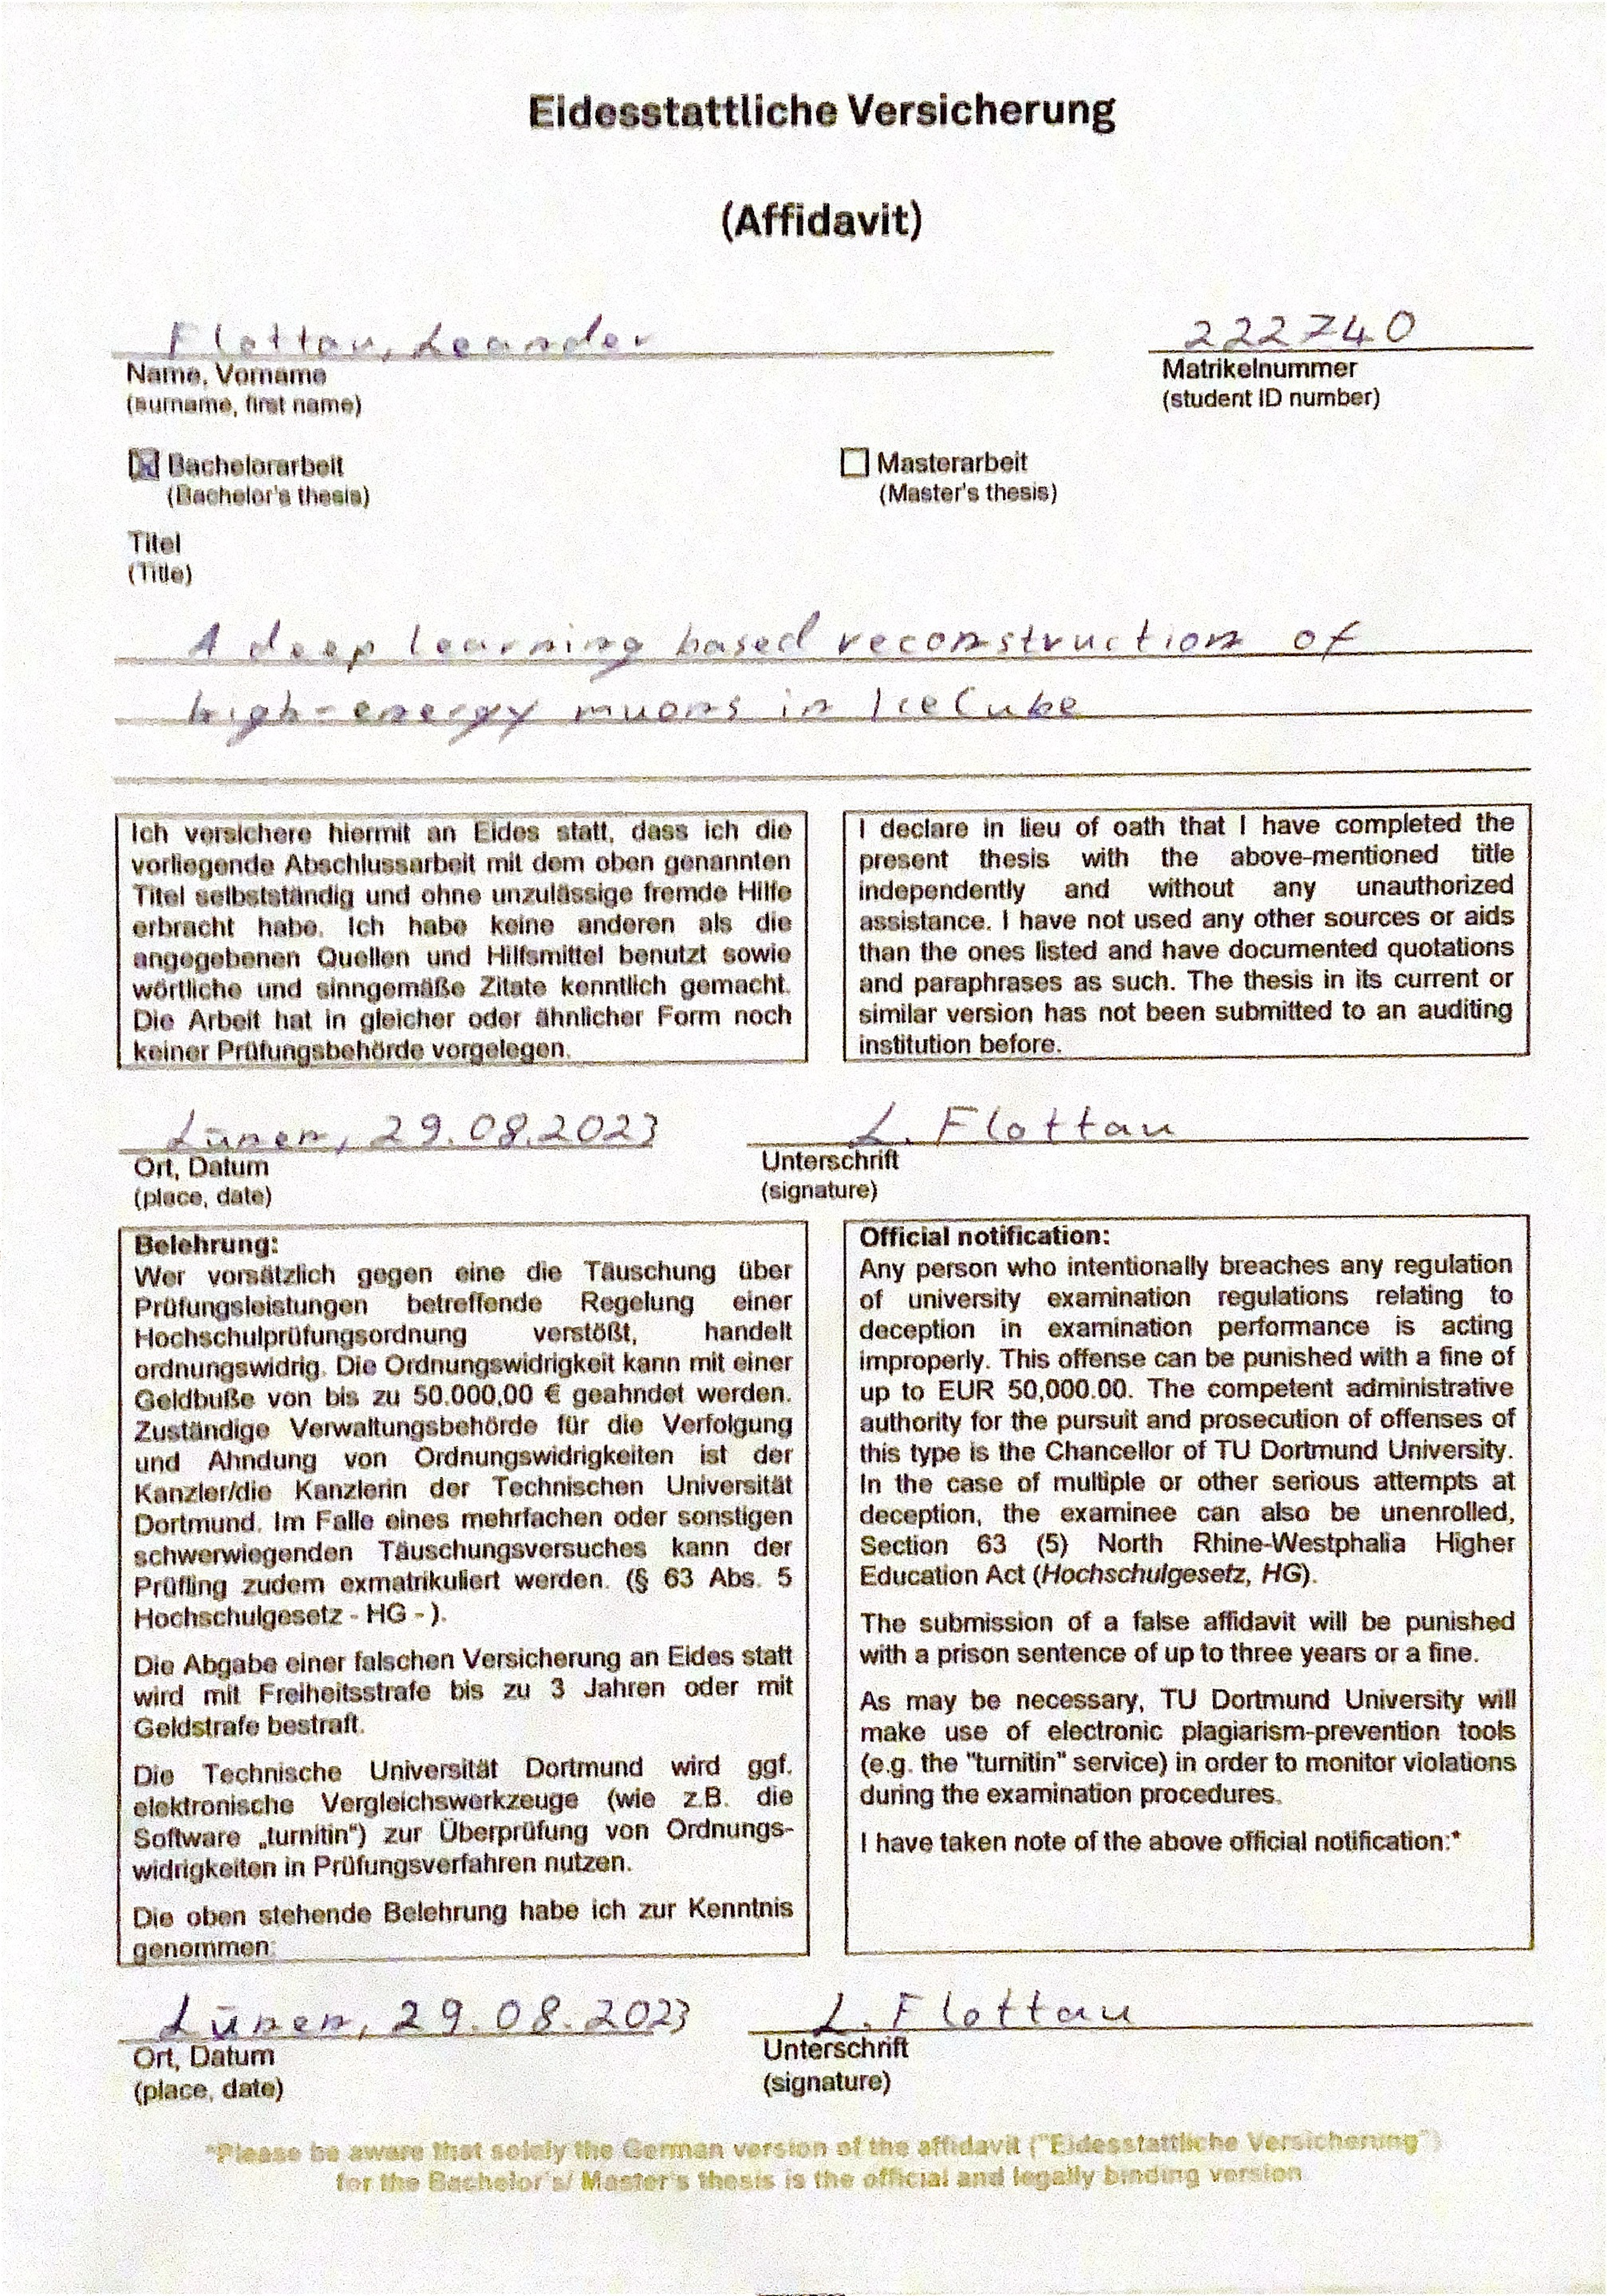
\includepdf{content/Eidesstattliche Versicherung unterschrieben.pdf}

\end{document}